% !TEX TS-program = XeLaTeX
% Command for running this example (needs latexmkrc file):
%    latexmk -bibtex -pdf main.tex

%	نمونه پایان‌نامه آماده شده با استفاده از کلاس tehran-thesis، نگارش 1
%	سینا ممکن، دانشگاه تهران 
%	https://github.com/sinamomken/tehran-thesis
%	گروه پارسی‌لاتک
%	http://www.parsilatex.com
%	این نسخه، بر اساس نسخه‌ 0.1 از کلاس IUST-Thesis آقای محمود امین‌طوسی آماده شده است.
%        http://profsite.sttu.ac.ir/mamintoosi

%----------------------------------------------------------------------------------------------
% اگر قصد نوشتن پروژه کارشناسی را دارید، در خط زیر به جای msc، کلمه bsc و اگر قصد نوشتن رساله دکترا را دارید، کلمه phd را قرار دهید. کلیه تنظیمات لازم، به طور خودکار، اعمال می‌شود.

% اگر مایلید پایان‌نامه شما دورو باشد به جای oneside در خط زیر از twoside استفاده کنید.

% برای حاشیه‌نویسی و کم کردن صفحات ابتدایی، گزینه draft را وارد و برای نسخه نهایی آن را حذف کنید.

% برای استفاده از قلم‌های سری IR Series گزینه irfonts را وارد و برای استفاده از قلم‌های X Series 2 آن را حذف کنید.

\documentclass[
oneside
,openany
,bsc
,irfonts
% ,draft
]{./tex/tehran-thesis}

% فایل commands.tex را مطالعه کنید؛ چون دستورات مربوط به فراخوانی بسته‌ها، فونت و دستورات خاص در این فایل قرار دارد.
% در این فایل، دستورها و تنظیمات مورد نیاز، آورده شده است.
%-------------------------------------------------------------------------------------------------------------------
% دستوراتی که پوشه پیش‌فرض زیرفایل‌های tex را مشخص می‌کند.
%\makeatletter
%\def\input@path{{./tex/}}
%\makeatother
% در ورژن جدید زی‌پرشین برای تایپ متن‌های ریاضی، این سه بسته، حتماً باید فراخوانی شود
\usepackage{amsthm,amssymb,amsmath}
% بسته‌ای برای تنطیم حاشیه‌های بالا، پایین، چپ و راست صفحه
\usepackage[top=40mm, bottom=40mm, left=25mm, right=35mm]{geometry}
% بسته‌‌ای برای ظاهر شدن شکل‌ها و تعیین آدرس تصاویر
\usepackage[final]{graphicx}
\graphicspath{{./img/}}
% بسته‌های مورد نیاز برای نوشتن کدها، رنگ‌آمیزی آنها و تعیین پوشهٔ کدها
\usepackage[final]{listings}
\usepackage[usenames,dvipsnames,svgnames,table]{xcolor}
\lstset{inputpath=./code/}
% بسته‌ای برای رسم کادر
\usepackage{framed} 
% بسته‌‌ای برای چاپ شدن خودکار تعداد صفحات در صفحه «معرفی پایان‌نامه»
\usepackage{lastpage}
% بسته‌ٔ لازم برای: ۱. تغییر شماره‌گذاری صفحات پیوست. ۲. تصحیح باگ آدرس وب حاوی '%' در مراجع
\usepackage{etoolbox}

\usepackage{protobuf/lang}  % include language definition for protobuf
\usepackage{protobuf/style} % include custom style for proto declarations.

\usepackage[utf8]{inputenc}
\usepackage{textcomp}
\usepackage{pgfplots}
\pgfplotsset{width=10cm,compat=1.9}

%%%%%%%%%%%%%%%%%%%%%%%%%%%%%%%%%%%%
%%% دستورات وابسته به استیل مراجع:
%% اگر از استیل‌های natbib (plainnat-fa، asa-fa، chicago-fa) استفاده می‌کنید، خط زیر را فعال و بعدی‌اش را غیرفعال کنید.
%\usepackage{natbib}
%\newcommand{\citelatin}[1]{\cite{#1}\LTRfootnote{\citeauthor*{#1}}}
%\newcommand{\citeplatin}[1]{\citep{#1}\LTRfootnote{\citeauthor*{#1}}}
%% اگر از سایر استیل‌ها استفاده می‌کنید، خط بالا را غیرفعال و خط‌های زیر را فعال کنید.
\let\citep\cite
\let\citelatin\cite
\let\citeplatin\cite
%%%%%%%%%%%%
% بررسی حالت پیش نویس
\usepackage{ifdraft}
\ifdraft
{%
	% بسته‌ٔ ایجاد لینک‌های رنگی با امکان جهش
	\usepackage[unicode=true,pagebackref=true,
colorlinks,linkcolor=blue,citecolor=blue,final]{hyperref}
	%\usepackage{todonotes}
	\usepackage[firstpage]{draftwatermark}
	\SetWatermarkText{\ \ \ پیش‌نویس}
	\SetWatermarkScale{1.2}
}
{ 
	\usepackage[pagebackref=false,colorlinks,
	linkcolor=blue,citecolor=blue,urlcolor=blue]{hyperref}
	%\usepackage[disable]{todonotes} % final without TODOs
}

\usepackage[obeyDraft]{todonotes}
\setlength{\marginparwidth}{2cm}

%%%%%%%%%%%%
%%% تصحیح باگ: اگر در مراجع، آدرس وب حاوی '%' بوده و pagebackref فعال باشد، دستورات زیر باید بیایند:
%% برای استیل‌های natbib مثل plainnat-fa، asa-fa، chicago-fa
\makeatletter
\let\ORIG@BR@@lbibitem\BR@@lbibitem
\apptocmd\ORIG@BR@@lbibitem{\endgroup}{}{}
\def\BR@@lbibitem{\begingroup\catcode`\%=12 \ORIG@BR@@lbibitem}
\makeatother
%% برای سایر استیل‌ها
\makeatletter
\let\ORIG@BR@@bibitem\BR@@bibitem
\apptocmd\ORIG@BR@@bibitem{\endgroup}{}{}
\def\BR@@bibitem{\begingroup\catcode`\%=12 \ORIG@BR@@bibitem}
\makeatother
%%%%%%%%%%%%%%%%%%%%%%%%%%%%%%%%%%%%

% بسته‌ لازم برای تنظیم سربرگ‌ها
\usepackage{fancyhdr}
%\usepackage{enumitem}
\usepackage{setspace}
% بسته‌های لازم برای نوشتن الگوریتم
\usepackage{algorithm}
\usepackage{algorithmic}
% بسته‌های لازم برای رسم بهتر جداول
\usepackage{tabulary}
\usepackage{tabularx}
\usepackage{rotating}
% بسته‌های لازم برای رسم تنظیم بهتر شکل‌ها و زیرشکل‌ها
\usepackage[export]{adjustbox}
\usepackage{subfig}
\usepackage[subfigure]{tocloft}
% بسته‌ای برای رسم نمودارها و نیز صفحه مالکیت اثر
\usepackage{tikz}
% بسته‌ای برای ظاهر شدن «مراجع» و «نمایه» در فهرست مطالب
\usepackage[nottoc]{tocbibind}
% دستورات مربوط به ایجاد نمایه
\usepackage{makeidx}
\makeindex
%%% بسته ایجاد واژه‌نامه با xindy
\usepackage[xindy,toc,acronym,nonumberlist=true]{glossaries}

% بسته زیر باگ ناشی از فراخوانی بسته‌های زیاد را برطرف می‌کند.
\usepackage{morewrites}
%%%%%%%%%%%%%%%%%%%%%%%%%%
% فراخوانی بسته زی‌پرشین (باید آخرین بسته باشد)
\usepackage[extrafootnotefeatures, localise=on, displaymathdigits=persian]{xepersian}




\makeatletter
% تعریف قلم فارسی و انگلیسی و مکان قلم‌ها
\if@irfonts
\settextfont[Path={./font/}, BoldFont={IRLotusICEE_Bold.ttf}, BoldItalicFont={IRLotusICEE_BoldIranic.ttf}, ItalicFont={IRLotusICEE_Iranic.ttf},Scale=1.2]{IRLotusICEE.ttf}
% LiberationSerif or FreeSerif as free equivalents of Times New Roman
\setlatintextfont[Path={./font/}, BoldFont={LiberationSerif-Bold.ttf}, BoldItalicFont={LiberationSerif-BoldItalic.ttf}, ItalicFont={LiberationSerif-Italic.ttf},Scale=1]{LiberationSerif-Regular.ttf}
% چنانچه می‌خواهید اعداد در فرمول‌ها، انگلیسی باشد، خط زیر را غیرفعال کنید
% و گزینهٔ displaymathdigits=persian را از خط ۱۰۹ حذف کنید.
\setdigitfont[Path={./font/}, Scale=1.2]{IRLotusICEE.ttf}
% تعریف قلم‌های فارسی و انگلیسی اضافی برای استفاده در بعضی از قسمت‌های متن
\setiranicfont[Path={./font/}, Scale=1.3]{IRLotusICEE_Iranic.ttf}				% ایرانیک، خوابیده به چپ
\setmathsfdigitfont[Path={./font/}]{IRTitr.ttf}
\defpersianfont\titlefont[Path={./font/}, Scale=1]{IRTitr.ttf}
% برای تعریف یک قلم خاص عنوان لاتین، خط بعد را فعال و ویرایش کنید و خط بعد از آن را غیرفعال کنید.
% \deflatinfont\latintitlefont[Scale=1]{LiberationSerif}
\font\latintitlefont=cmssbx10 scaled 2300 %cmssbx10 scaled 2300
\else
\settextfont{XB Niloofar}
\setlatintextfont{Junicode}
% چنانچه می‌خواهید اعداد در فرمول‌ها، انگلیسی باشد، خط زیر را غیرفعال کنید
% و گزینهٔ displaymathdigits=persian را از خط ۱۰۹ حذف کنید.
\setdigitfont{XB Niloofar}
% تعریف قلم‌های فارسی و انگلیسی اضافی برای استفاده در بعضی از قسمت‌های متن
% \setmathsfdigitfont{XB Titre}
\defpersianfont\titlefont{XB Titre}
\deflatinfont\latintitlefont[Scale=1.1]{Junicode}
\fi
\makeatother

% برای استفاده از قلم نستعلیق خط بعد را فعال کنید.
% \defpersianfont\nastaliq[Scale=1.2]{IranNastaliq}


%%%%%%%%%%%%%%%%%%%%%%%%%%
% راستچین شدن todonotes
\presetkeys{todonotes}{align=right,textdirection=righttoleft}{}
\makeatletter
\providecommand\@dotsep{5}
\def\listtodoname{فهرست کارهای باقیمانده}
\def\listoftodos{\noindent{\Large\vspace{10mm}\textbf{\listtodoname}}\@starttoc{tdo}}
\renewcommand{\@todonotes@MissingFigureText}{شکل}
\renewcommand{\@todonotes@MissingFigureUp}{شکل}
\renewcommand{\@todonotes@MissingFigureDown}{جاافتاده}
\makeatother
% دستوری برای حذف کلمه «چکیده»
\renewcommand{\abstractname}{}
% دستوری برای حذف کلمه «abstract»
%\renewcommand{\latinabstract}{}
% دستوری برای تغییر نام کلمه «اثبات» به «برهان»
\renewcommand\proofname{\textbf{برهان}}
% دستوری برای تغییر نام کلمه «کتاب‌نامه» به «مراجع»
\renewcommand{\bibname}{مراجع}
% دستوری برای تعریف واژه‌نامه انگلیسی به فارسی
\newcommand\persiangloss[2]{#1\dotfill\lr{#2}\\}
% دستوری برای تعریف واژه‌نامه فارسی به انگلیسی 
\newcommand\englishgloss[2]{#2\dotfill\lr{#1}\\}
% تعریف دستور جدید «\پ» برای خلاصه‌نویسی جهت نوشتن عبارت «پروژه/پایان‌نامه/رساله»
\newcommand{\پ}{پروژه/پایان‌نامه/رساله }

%\newcommand\BackSlash{\char`\\}

%%%%%%%%%%%%%%%%%%%%%%%%%%
% \SepMark{-}

% تعریف و نحوه ظاهر شدن عنوان قضیه‌ها، تعریف‌ها، مثال‌ها و ...
\theoremstyle{definition}
\newtheorem{definition}{تعریف}[section]
\theoremstyle{theorem}
\newtheorem{theorem}[definition]{قضیه}
\newtheorem{lemma}[definition]{لم}
\newtheorem{proposition}[definition]{گزاره}
\newtheorem{corollary}[definition]{نتیجه}
\newtheorem{remark}[definition]{ملاحظه}
\theoremstyle{definition}
\newtheorem{example}[definition]{مثال}

%\renewcommand{\theequation}{\thechapter-\arabic{equation}}
%\def\bibname{مراجع}
\numberwithin{algorithm}{chapter}
\def\listalgorithmname{فهرست الگوریتم‌ها}
\def\listfigurename{فهرست تصاویر}
\def\listtablename{فهرست جداول}

%%%%%%%%%%%%%%%%%%%%%%%%%%%%
%%% دستورهایی برای سفارشی کردن سربرگ صفحات:
%\newcommand{\SetHeader}[1]{
% دستور زیر معادل با گزینه twoside است.
%\csname@twosidetrue\endcsname
\pagestyle{fancy}
%% دستورات زیر سبک صفحات fancy را تغییر می‌دهد:
% O=Odd, E=Even, L=Left, R=Right
% در صورت oneside بودن، عنوان فصل، سمت چپ ظاهر می‌شود.
\fancyhead{}
\fancyhead[OL]{\small\leftmark}
\fancyhead[ER]{\small\leftmark}
\fancyhead[OR]{\footnotesize\rightmark}
\fancyhead[EL]{\footnotesize\rightmark}
\renewcommand{\headrulewidth}{0.75pt}
% شکل‌دهی شماره و عنوان فصل در سربرگ
\renewcommand{\chaptermark}[1]{\markboth{فصل~\thechapter:\ #1}{}}
\makeatletter
\renewcommand{\rightmark}[1]{\@title}
\makeatother
%}
%%%%%%%%%%%%%%%%%%%%%%%%%%%%
%\def\MATtextbaseline{1.5}
%\renewcommand{\baselinestretch}{\MATtextbaseline}
\doublespacing
%%%%%%%%%%%%%%%%%%%%%%%%%%%%%
% دستوراتی برای اضافه کردن کلمه «فصل» در فهرست مطالب

\newlength\mylenprt
\newlength\mylenchp
\newlength\mylenapp

\renewcommand\cftpartpresnum{\partname~}
\renewcommand\cftchappresnum{\chaptername~}
\renewcommand\cftchapaftersnum{:}

\settowidth\mylenprt{\cftpartfont\cftpartpresnum\cftpartaftersnum}
\settowidth\mylenchp{\cftchapfont\cftchappresnum\cftchapaftersnum}
\settowidth\mylenapp{\cftchapfont\appendixname~\cftchapaftersnum}
\addtolength\mylenprt{\cftpartnumwidth}
\addtolength\mylenchp{\cftchapnumwidth}
\addtolength\mylenapp{\cftchapnumwidth}

\setlength\cftpartnumwidth{\mylenprt}
\setlength\cftchapnumwidth{\mylenchp}	

\makeatletter
{\def\thebibliography#1{\chapter*{\refname\@mkboth
   {\uppercase{\refname}}{\uppercase{\refname}}}\list
   {[\arabic{enumi}]}{\settowidth\labelwidth{[#1]}
   \rightmargin\labelwidth
   \advance\rightmargin\labelsep
   \advance\rightmargin\bibindent
   \itemindent -\bibindent

   \listparindent \itemindent
   \parsep \z@
   \usecounter{enumi}}
   \def\newblock{}
   \sloppy
   \sfcode`\.=1000\relax}}
   
%اگر مایلید در شماره گذاری حرفی و ابجد به جای آ از الف استفاده شود دستورات زیر را فعال کنید.   
%\def\@Abjad#1{%
%  \ifcase#1\or الف\or ب\or ج\or د%
%           \or هـ\or و\or ز\or ح\or ط%
%           \or ی\or ک\or ل\or م\or ن%
%           \or س\or ع\or ف\or ص%
%           \or ق\or ر\or ش\or ت\or ث%
%            \or خ\or ذ\or ض\or ظ\or غ%
%            \else\@ctrerr\fi}
%
% \def\abj@num@i#1{%
%   \ifcase#1\or الف\or ب\or ج\or د%
%            \or هـ‍\or و\or ز\or ح\or ط\fi

%   \ifnum#1=\z@\abjad@zero\fi}   
%  
%   \def\@harfi#1{\ifcase#1\or الف\or ب\or پ\or ت\or ث\or

% ج\or چ\or ح\or خ\or د\or ذ\or ر\or ز\or ژ\or س\or ش\or ص\or ض\or ط\or ظ\or ع\or غ\or

% ف\or ق\or ک\or گ\or ل\or م\or ن\or و\or ه\or ی\else\@ctrerr\fi}

%
\makeatother

%%% امکان درج کد در سند
% در این قسمت رنگ، قلم و قالب‌بندی قسمت‌های مختلف یک کد تعیین می‌شود. 
\lstdefinestyle{myStyle}{
	basicstyle=\ttfamily, % whole listing /w verbatim font
	keywordstyle=\color{blue}\bfseries, % bold black keywords
	identifierstyle=, % nothing happens
	commentstyle=\color{LimeGreen}, % green comments
	stringstyle=\ttfamily\color{red}, % red typewriter font for strings
	showstringspaces=false % no special string spaces
	breaklines=true,
	breakatwhitespace=false,
	numbers=right, % line number formats
	numberstyle=\footnotesize\lr,
	numbersep=-10pt,
	frame=single,
	captionpos=b,
	captiondirection=RTL
}
\lstset{style=myStyle} % command to set default style
\def\lstlistingname{\rl{برنامهٔ}}
\def\lstlistlistingname{\rl{فهرست برنامه‌ها}}


% for numbering subsubsections
\setcounter{secnumdepth}{3}
%to include subsubsections in the table of contents
\setcounter{tocdepth}{3}


% مشخصات پایان‌نامه را در فایلهای faTitle و enTitle وارد نمایید.
% !TeX root=../main.tex
% در این فایل، عنوان پایان‌نامه، مشخصات خود، متن تقدیمی‌، ستایش، سپاس‌گزاری و چکیده پایان‌نامه را به فارسی، وارد کنید.
% توجه داشته باشید که جدول حاوی مشخصات پروژه/پایان‌نامه/رساله و همچنین، مشخصات داخل آن، به طور خودکار، درج می‌شود.
%%%%%%%%%%%%%%%%%%%%%%%%%%%%%%%%%%%%
% دانشگاه خود را وارد کنید
\university{دانشگاه تهران}
% پردیس دانشگاهی خود را اگر نیاز است وارد کنید (مثال: فنی، علوم پایه، علوم انسانی و ...)
\college{پردیس دانشکده‌های فنی}
% دانشکده، آموزشکده و یا پژوهشکده  خود را وارد کنید
\faculty{دانشکده مهندسی برق و کامپیوتر}
% گروه آموزشی خود را وارد کنید (در صورت نیاز)
\department{گروه مهندسی نرم‌افزار}
% رشته تحصیلی خود را وارد کنید
\subject{مهندسی کامپیوتر}
% گرایش خود را وارد کنید
\field{مهندسی نرم‌افزار}
% عنوان پایان‌نامه را وارد کنید
\title{درستی‌سنجی نرم‌افزارهای با معماری میکروسرویس}
% نام استاد(ان) راهنما را وارد کنید
\firstsupervisor{دکتر حسین حجت}
\firstsupervisorrank{استاد}
%\secondsupervisor{دکتر راهنمای دوم}
%\secondsupervisorrank{استادیار}
% نام استاد(دان) مشاور را وارد کنید. چنانچه استاد مشاور ندارید، دستورات پایین را غیرفعال کنید.
%\firstadvisor{دکتر مشاور اول}
%\firstadvisorrank{استادیار}
%\secondadvisor{دکتر مشاور دوم}
% نام داوران داخلی و خارجی خود را وارد نمایید.
%\internaljudge{دکتر داور داخلی}
%\internaljudgerank{دانشیار}
%\externaljudge{دکتر داور خارجی}
%\externaljudgerank{دانشیار}
%\externaljudgeuniversity{دانشگاه داور خارجی}
% نام نماینده کمیته تحصیلات تکمیلی در دانشکده \ گروه
%\graduatedeputy{دکتر نماینده}
%\graduatedeputyrank{دانشیار}
% نام دانشجو را وارد کنید
\name{شایان}
% نام خانوادگی دانشجو را وارد کنید
\surname{حسینی}
% شماره دانشجویی دانشجو را وارد کنید
\studentID{810194540}
% تاریخ پایان‌نامه را وارد کنید
\thesisdate{شهریور ۱۳۹۹}
% به صورت پیش‌فرض برای پایان‌نامه‌های کارشناسی تا دکترا به ترتیب از عبارات «پروژه»، «پایان‌نامه» و «رساله» استفاده می‌شود؛ اگر  نمی‌پسندید هر عنوانی را که مایلید در دستور زیر قرار داده و آنرا از حالت توضیح خارج کنید.
%\projectLabel{پایان‌نامه}

% به صورت پیش‌فرض برای عناوین مقاطع تحصیلی کارشناسی تا دکترا به ترتیب از عبارت «کارشناسی»، «کارشناسی ارشد» و «دکتری» استفاده می‌شود؛ اگر نمی‌پسندید هر عنوانی را که مایلید در دستور زیر قرار داده و آنرا از حالت توضیح خارج کنید.
%\degree{}
%%%%%%%%%%%%%%%%%%%%%%%%%%%%%%%%%%%%%%%%%%%%%%%%%%%%
%% پایان‌نامه خود را تقدیم کنید! %%
%\dedication
%{
%{\Large تقدیم به:}\\
%\begin{flushleft}{
%	\huge
%	همسر و فرزندانم\\
%	\vspace{7mm}
%	و\\
%	\vspace{7mm}
%	پدر و مادرم
%}
%\end{flushleft}
%}
%% متن قدردانی %%
%% ترجیحا با توجه به ذوق و سلیقه خود متن قدردانی را تغییر دهید.
\acknowledgement{
سپاس خداوندگار حکیم را که با لطف بی‌کران خود، آدمی را به زیور عقل آراست.

در آغاز وظیفه‌  خود  می‌دانم از زحمات بی‌دریغ اساتید  راهنمای خود،  جناب آقای دکتر حجت، صمیمانه تشکر و  قدردانی کنم که در طول انجام این پایان‌نامه با نهایت صبوری همواره راهنما و مشوق من بودند و قطعاً بدون راهنمایی‌های ارزنده‌ ایشان، این مجموعه به انجام نمی‌رسید.

%از همکاری و مساعدت‌های دکتر ... مسئول تحصیلات تکمیلی و سایر کارکنان دانشکده بویژه سرکار خانم ... کمال تشکر را دارم.

%با سپاس بی‌دریغ خدمت دوستان گران‌مایه‌ام، خانم‌ها ... و آقایان ... در آزمایشگاه ...، که با همفکری مرا صمیمانه و مشفقانه یاری داده‌اند.

و در پایان، تشکر می‌کنم از خانواده عزیزم که پشتیبان من بودند.
}
%%%%%%%%%%%%%%%%%%%%%%%%%%%%%%%%%%%%
%چکیده پایان‌نامه را وارد کنید
\fa-abstract{
امروزه بسیاری از برنامه‌های بزرگ توسط تعداد زیادی از 
\glspl{Microservice}
ساخته می‌شوند. هر کدام از این میکروسرویس‌ها در محیطی از بقیه مستقر می‌شود و با دیگر میکروسرویس‌ها از طریق
\gls{RemoteProcedureCall}
ارتباط برقرار می‌کند. استفاده از میکروسرویس‌ها سبب بهبود مقیاس‌پذیری - هر کدام از اجزای یک برنامه می‌توانند به طور مستقل رشد کنند - و استقرار می‌شود. اما این برنامه‌ به طور ذاتی توزیع‌شده هستند و ابزارهای فعلی این قابلیت را ندارند که بتوان درباره این برنامه‌ها استدلال کرد و یا از رفتارهای آن‌ها به طور کلی اطمینان حاصل کرد.
در این پروژه ما سیستمی را معرفی می‌کنیم تا با استفاده از آن بتوان ارتباط میان میکروسرویس‌ها درستی‌سنجی کرد. با الهام گرفتن از
\gls{DesignByContract}
، سیستم ما سرویس‌ها را در هنگام اجرا دیده‌بانی می‌کند تا سرویس‌هایی را که به قرارداد خود پایبند نیستند را پیدا کند. در نهایت، ما این سیستم را روی یک برنامه با معماری میکروسرویس پیاده می‌کنیم و نشان می‌دهیم که چگونه ایراداتی را در این برنامه پیدا کردیم بدون اینکه کارایی برنامه کاهش پیدا کند.

}
% کلمات کلیدی پایان‌نامه را وارد کنید
\keywords{درستی‌سنجی، میکروسرویس، طراحی بر اساس قرارداد}
% انتهای وارد کردن فیلد‌ها
%%%%%%%%%%%%%%%%%%%%%%%%%%%%%%%%%%%%%%%%%%%%%%%%%%%%%%

% مشخصات انگلیسی پایان‌نامه
% !TeX root=../main.tex
% در این فایل، عنوان پایان‌نامه، مشخصات خود و چکیده پایان‌نامه را به انگلیسی، وارد کنید.

%%%%%%%%%%%%%%%%%%%%%%%%%%%%%%%%%%%%
\latinuniversity{University of Tehran}
\latincollege{College of Engineering}
\latinfaculty{Faculty of Electrical and Computer Engineering}
\latindepartment{Software Engineering}
\latinsubject{Computer Engineering}
\latinfield{Software Engineering}
\latintitle{Verification of Microservices}
\firstlatinsupervisor{Dr. Hossein Hojjat}
%\secondlatinsupervisor{Second Supervisor}
%\firstlatinadvisor{First Advisor}
%\secondlatinadvisor{Second Advisor}
\latinname{Shayan}
\latinsurname{Hosseini}
\latinthesisdate{September 2020}
\latinkeywords{Verification, Microservices, Contracts}
\en-abstract{
Many large applications are now built using collections of
microservices, each of which is deployed in isolated containers 
and which interact with each other through the use
of remote procedure calls (RPCs). The use of microservices
improves scalability – each component of an application can
be scaled independently – and deployability. However, such
applications are inherently distributed and current tools do not
provide mechanisms to reason about and ensure their global
behavior.
In this project, we propose a system to verify microservices communications.
Inspired by Design by Contract, our system monitor services at runtime to detect
services that do not satisfy their contracts. Finally, we implement our system on
some real-world microservices system and we show how we found some bugs in these systems
without performance loss.
}


% تنظیمات و تعاریف واژه‌نامه و اختصارات
\input{./tex/glossaries-settings}

%%%% A
\newword{Gloss}{Glossary}{واژه‌نامه}{واژه‌نامه‌ها}

\newword{Acronym}{Acronym}{اختصار}{اختصارات}

\newword{Description}{Description}{توصیف}{توصیف‌ها}

\newword{Draft}{Draft}{پیش‌نویس}{پیش‌نویس‌ها}

\newword{Absorption}{Absorption}{جذب}{جذب‌ها}

\newword{RandomVariable}{Random Variable}
{متغیر تصادفی}{متغیرهای تصادفی}

\newword{Action}{Action}
{کنش}{کنش‌ها}

\newword{Optimization}{Optimization}{بهینه‌سازی}{}

\newword{RemoteProcedureCall}{Remote Procedure Call}
{فراخوانی از راه دور}{فراخوانی‌های از راه دور}

\newword{DesignByContract}{Design by Contract}
{طراحی به‌وسیله قرارداد}{طراحی به‌وسیله قراردادها}

%\newacronym{a}{$a$}{شتاب (m/s$^2$)}
\newacronym{F}{$F$}{نیرو (N)}
\newacronym{RPC}{$RPC$}{\lr{Remote Procedure Call}}
\newacronym{SOA}{$SOA$}{\lr{Service Oriented Architecture}}


\begin{document}

\pagenumbering{adadi} % یک، دو، ...
% ابتدای درج صفحات مختلف
\titlePage
% بررسی حالت پیش‌نویس
\ifoptiondraft{}{% 
    \besmPage
    %\titlePage
    %\davaranPage
%%%%%%%%%%%%%%%%%%%%%%%%%%%%
% در این قسمت اسامی اساتید راهنما، مشاور و داور باید به صورت دستی وارد شوند
%\renewcommand{\arraystretch}{1.2}


%%%%%%%%%%%%%%%%%%%%%%%%%%%
    \esalatPage
    %\mojavezPage
% چنانچه مایل به چاپ صفحات «تقدیم»، «نیایش» و «سپاس‌گزاری» در خروجی نیستید، خط‌های زیر را با گذاشتن ٪  در ابتدای آنها غیرفعال کنید.
    %\taghdimPage
    \ghadrdaniPage
} % end ifoptiondraft
\abstractPage
% شروع درج فهرست‌ها
\newpage\clearpage
\pagenumbering{harfi} % آ، ب، ...
\tableofcontents \newpage
% بررسی حالت پیش‌نویس برای بقیه فهرست‌ها
\ifoptiondraft{
    \listoftodos
}{%
    \listoffigures \newpage
    \listoftables  \newpage
    \addcontentsline{toc}{chapter}{\listalgorithmname}
    \listofalgorithms %\newpage
    \addcontentsline{toc}{chapter}{\lstlistlistingname}
    \lstlistoflistings \newpage
    \printacronyms
} % end ifoptiondraft


\pagestyle{fancy}
\pagenumbering{arabic} % 1, 2, ...

% !TeX root=../main.tex

\chapter{مقدمه و بیان مساله}
% دستور زیر باعث عدم‌نمایش شماره صفحه در اولین صفحه‌ی این فصل می‌شود.
%\thispagestyle{empty}
\section{مقدمه}
هر روزه برنامه‌های بیشتری تحت وب ساخته می‌شود که به صورت کاملا مستقل از هم مستقر می‌شوند و با استفاده از
\gls{RPC}
با هم ارتباط برقرار می‌کنند. پیدایش روش‌های کم‌هزینه مجازی‌سازی (برای مثال
\glspl{Container})
امکان به کارگیری تعداد زیادی سرویس ریزدانه را فراهم کرده‌اند که آن‌ها را میکروسرویس می‌نامند. شکستن برنامه‌ها به این شکل سودهای بسیاری خواهد داشت:‌ در این صورت مقیاس‌پذیری ساده می‌شود (هر سرویس به طور مستقل می‌تواند رشد کند)،‌ انعطاف‌پذیری بیشتری در تخصیص منابع و زمان ارائه می‌شود، امکان استفاده مجدد از کدها بیشتر می‌شود، امکان استفاده از روش‌های جدید تحمل خطا به وجود خواهد آمد، و امکان استفاده از سرویس‌های خارجی مانند
\lr{Amazon S3}
میسر می‌شود. در نتیجه این معماری توسط تعداد زیادی از شرکت‌های بزرگ و استارتاپ‌ها استفاده می‌شود (برای مثال
\lr{Uber} \cite{toddhoff2020}
و
\lr{Netflix} \cite{tonymauro2020})
و همینطور در مقیاس‌های بسیار بزرگی نیز استقرار یافته است (برای مثال برنامه شرکت
\lr{Uber} \cite{toddhoff2020}
از بیش از ۱۰۰۰ میکروسرویس تشکیل شده است).

در این تحقیق ما قصد داریم تا امکان درستی‌سنجی برنامه‌های مبتنی بر معماری میکروسرویس را بررسی کنیم و روشی برای انجام این کار ارائه دهیم.

\section{تاریخچه‌ای از موضوع تحقیق}
معماری میکروسرویس یک معماری بسیار جدید است که در چند سال اخیر به سبب رشد سریع برنامه‌های تحت وب شکل گرفته است. به همین سبب کارهای زیادی روی درستی‌سنجی برنامه‌های با این معماری صورت نگرفته است. در اینجا ما از بررسی روش‌های درستی‌سنجی سیستم‌های توزیع‌شده صرف نظر می‌کنیم و فقط روی درستی‌سنجی نرم‌افزارهای با معماری میکروسرویس تمرکز خواهیم کرد.

سیستم
ucheck \cite{panda2017verification}
یک سیستم برای درستی‌سنجی میکروسرویس‌ها است. این سیستم،‌ به صورت جدا از میکروسرویس‌ها مستقر می‌شود و با مانیتور کردن ترافیک شبکه و پیام‌های رد و بدل شده، سعی در بررسی درستی شرط‌های تعریف شده را دارد. این سیستم از استدلال
\lr{rely-guarantee} \cite{Jones83}
برای شرط‌ها استفاده می‌کند. به دلیل پیچیدگی پیاده‌سازی تحلیل ترافیک شبکه، این سیستم هیچ پیاده‌سازی در دسترسی ندارد. همینطوری استدلال
\lr{rely-guarantee}
برای بررسی دقیق سیستم‌های توزیع‌شده طراحی شده و نوشتن شرط‌های مناسب در آن، کاری بسیار دشوار است.

سیستم
Whip \cite{waye2017whip}
یک سیستم دیگر برای درستی‌سنجی میکروسرویس‌هاست. این سیستم هم مانند ucheck سعی می‌کند تا با تحلیل ترافیک شبکه عمل درستی‌سنجی را انجام دهد و به همین علت پیاده‌سازی مناسب استفاده عملیاتی ندارد. Whip از قراردادها برای توصیف شرط‌ها استفاده می‌کند و روشی برای توصیف قراردادهای سطح‌ بالا ارائه می‌دهد که از آن برای
\gls{BlameAssignment}
دقیق‌تر استفاده می‌کند.

\section{شرح مسئله تحقیق}
با بزرگ شدن اندازه برنامه و بیشتر شدن پیچیدگی‌های آن، اطمینان از درستی این برنامه‌های مبتنی بر معماری میکروسرویس برای گردانندگان آن سخت‌تر می‌شود. ویژگی‌های این برنامه‌ها، وابسته است به رفتار هر کدام از میکروسرویس‌های تشکیل دهنده آن، و تنظیمات مربوط به ارتباطات بین آن‌ها. فهمیدن برقراری یک شرط خاص در هنگام اجرای یک برنامه یک مساله غیربدیهی برای برنامه‌های کوچک است، اما برای برنامه بزرگی که از تعدادی زیاد میکروسرویس تشکیل شده است، بسیار سخت است. برای مثال، یک برنامه ساده را در نظر بگیرید که از سه سرویس تشکیل شده است: یک وب‌سرور، یک سرویس احراز هویت و یک پایگاه داده. اطمینان از این شرط که تنها کاربرانی که احراز هویت آن‌ها تایید شده است، می‌توانند پایگاه داده را به‌روزرسانی کنند، نیازمند دسترسی به وضعیت وب‌سرور (برای تعیین درخواستی که موجب به‌روزرسانی شده است) و سرویس احراز هویت (برای بررسی احراز هویت درخواست‌دهنده)‌ علاوه بر نیازمندی دسترسی به پایگاه داده است. حتی اگر تمامی میکروسرویس‌ها هم روش‌هایی را برای دسترسی به وضعیت‌شان ارائه کنند، باز هم نیاز داریم تا آن‌ها را با هم هماهنگ کنیم تا یک تصویر نامتناقض از کل برنامه به دست آوردیم. استفاده از چنین روش‌هایی در برنامه‌های بزرگ، بسیار ناکارآمد خواهد بود.

\section{تعریف موضوع تحقیق}
در قسمت‌های قبل، به نیاز به درستی‌سنجی برنامه‌های با معماری میکروسرویس و پیچیدگی‌های آن اشاره شد. در این تحقیق ما روی موضوع درستی‌سنجی نرم‌افزارهای با معماری میکروسرویس تمرکز می‌کنیم. در این تحقیق ما سعی می‌کنیم که در یک برنامه‌ بزرگ با تعداد سرویس‌های بسیار زیاد، از برقراری شرط‌های مهمی که توسط کاربر تعیین می‌شوند، اطمینان حاصل کنیم.

\section{اهداف و آرمان‌های کلی تحقیق}
در این تحقیق ما یک روش برای درستی‌سنجی برنامه‌های با معماری میکروسرویس ارائه می‌کنیم به گونه‌ای که مشکلات تحقیقات قبلی را نداشته باشد. در این تحقیق ما روی درستی‌سنجی ارتباط بین میکروسرویس‌ها تمرکز می‌کنیم چرا که پیچیدگی اصلی در در این معماری، ارتباطات زیاد بین تعداد زیاد سرویس است که روی شبکه و با استفاده از
\gls{RPC}
با هم صحبت می‌کنند. همینطور به دلیل اینکه این مسئله، یک مسئله کاربردی مهندسی نرم‌افزار است، وجود یک پیاده‌سازی مناسب برای محیط‌های عملیاتی بخش مهمی از تحقیق است. به همین دلیل،‌ ارائه یک پیاده‌سازی مناسب از اهداف اصلی این تحقیق است.

\section{روش انجام تحقیق}
با توجه به اهداف گفته شده، ما استفاده از قراردادها را برای نوشتن شرط‌ها و بررسی آن‌ها انتخاب کردیم. طراحی توسط قرارداد روش قدرتمندی است که با استفاده از آن به خوبی می‌توان شرط‌های لازم را برای
\glspl{RemoteProcedureCall}
نوشت. ما این شرط‌ها در زمان اجرای برنامه بررسی می‌کنیم و در صورت نقض شدن هر شرط، آن را به توسعه‌دهنده اطلاع می‌دهیم. در این اشکالات در کل سیستم پخش نمی‌شوند و توسعه‌دهنده در اولین فرصت متوجه آن‌ها می‌شود. همچنین در روش ما این امکان وجود دارد که بتوان روی ترتیب اجرا
\gls{RPC}ها
شرط نوشت. این موضوع کمک می‌کند که بسیار بهتر بتوان ارتباط میان میکروسرویس‌ها را درستی‌سنجی کرد.

سپس برای روش ارائه شده، یک پیاده‌سازی در زبان برنامه‌نویسی
Go \cite{golang}
و برای چارچوب
gRPC \cite{grpc}
ارائه می‌دهیم و سپس با استفاده از آن به درستی‌سنجی یک برنامه با معماری میکروسرویس می‌پردازیم و نشان می‌دهیم که چگونه در آن اشکالاتی را پیدا کردیم. در نهایت سربار روشمان را روی کارایی برنامه بررسی می‌کنیم و نشان می‌دهیم که روش ما سربار بسیار کمی خواهد داشت.

\section{ساختار پایان‌نامه}
		% فصل اول: مقدمه
% !TeX root=../main.tex
\chapter{مفاهیم اولیه و پیش‌زمینه}
%\thispagestyle{empty} 

\section{مقدمه}
در این فصل برای روشن‌شدن مفاهیم و اصطلاحات حول موضوع این پژوهش، به تعریف برخی مفاهیم اساسی که پیش‌نیاز درک این پروژه هستند می‌پردازیم.

\section{معماری میکروسرویس}
میکروسرویس، همان طور که از نام آن مشخص می‌شود، اساساً به سرویس‌های نرم‌افزاری مستقلی گفته می‌شود که کارکردهای تجاری خاصی را در یک اپلیکیشن نرم‌افزاری ارائه می‌کنند. این سرویس‌ها می‌توانند به صورت مستقل از هم نگهداری، نظارت و توزیع شوند.

\gls{ServiceOrientedArchitecture}
به اپلیکیشن‌ها امکان ارتباط با یکدیگر روی یک رایانه منفرد و یا در زمان توزیع اپلیکیشن‌ها روی چندین رایانه در یک شبکه را ارائه می‌کند. هر میکروسرویس ارتباط اندکی با سرویس‌های دیگر دارد. این سرویس‌ها خودکفا هستند و یک کارکرد منفرد (یا گروهی از کارکردهای مشترک) را ارائه می‌کنند.

معماری میکروسرویس‌ها به طور طبیعی در سازمان‌های بزرگ و پیچیده استفاده می‌شود که در آن‌ها چند تیم توسعه می‌توانند مستقل از هم برای ارائه یک کارکرد تجاری کار بکنند و یا اپلیکیشن‌ها ملزم به ارائه خدمات به یک حوزه تجاری باشند.

پیش از آن که بخواهیم به توضیح مسائلی که میکروسرویس برای حل آن‌ها ابداع شده بپردازیم، باید تاریخچه تکامل نرم‌افزار را به طور خلاصه مرور کنیم.

\subsection{تکامل رایانه‌ها}
زمانی که رایانه‌ها برای اولین بار در دهه 1940 میلادی ارائه شدند، نرم‌افزار به صورت پانچ شده درون سخت‌افزارهای بزرگ و گران‌قیمت مانند کارت‌های پانچ و نوارهای پانچ جاسازی شده بود. دستورالعمل‌ها به زبان ماشین باینری نوشته شده بودند. متعاقباً اگر لازم می‌شد تغییری پیاده‌سازی شود، یک کارشناس زبان باینری ماشین باید دستورالعمل‌های جدید را در اختیار ماشین قرار می‌داد. این امر یک فرایند بسیار گران‌قیمت بود.

سپس نسل دوم رایانه‌ها در دهه 1950 میلادی به عنوان نسخه بهبود یافته نسل اول رایانه‌ها معرفی شدند. این رایانه‌ها به برنامه‌هایی با زبان اسمبلی نیاز داشتند که در تراشه‌های سخت‌افزاری کوچک‌تری نوشته می‌شد. فلسفه طراحی این رایانه‌ها پیرامون این واقعیت شکل گرفته بود که یادگیری زبان نمادین اسمبلی بسیار راحت‌تر از آموختن کدهای باینری است. در نتیجه اسمبلرها معرفی شدند که کد ماشین را به زبان نمادین اسمبلی تبدیل می‌کردند.

در این مورد نیز هر زمان که تغییری مورد نیاز بود، فرد باید دستورالعمل‌ها را در سخت‌افزار وارد می‌کرد. در نتیجه نرم‌افزار و سخت‌افزار باید از همدیگر جدا می‌شدند.

و سپس نسل سوم رایانه‌ها در دهه 1960 میلادی عرضه شدند. این رایانه‌ها به کامپایلر و مفسر برای ترجمه زبان قابل فهم از سوی انسان به کد ماشین نیاز داشتند. این رایانه‌ها کوچک‌تر بودند و می‌بایست نرم‌افزارهای قابل تعامل از سوی کاربر روی آن‌ها نصب می‌شد. نسل سوم رایانه‌ها می‌توانستند چندین اپلیکیشن را همزمان اجرا کنند. زبان‌های برنامه‌نویسی مختلفی معرفی شدند که روی این رایانه‌ها نصب می‌شدند. سخت‌افزار همچنان گران‌قیمت بود؛ اما انعطاف‌پذیری حاصل از جداسازی نرم‌افزار از سخت‌افزار موجب ایجاد فرصت‌های بی‌شماری برای بهبود کارکرد آن‌ها شد.

در نهایت نسل چهارم رایانه‌ها در دهه 1970 میلادی معرفی شدند. این رایانه‌ها دستگاه‌های دستی بودند که می‌توانستند در کف دست جای بگیرند. در این مورد نیز اپلیکیشن‌های جدید معرفی شدند که می‌توانستند روی دستگاه‌ها بدون نیاز به خرید سخت‌افزار جدید نصب شوند. سهولت نصب و قابلیت نگهداری موجب شد که بسیاری از شرکت‌ها بتوانند ایده‌های فناورانه جدیدی را ابداع کنند.

یک طرح مشترک وجود دارد. رایانه‌ها به این دلیل تکامل یافتند که همواره نیاز به نگهداری و بهبود اپلیکیشن‌های نصب شده روی رایانه‌ها وجود داشته است.

\subsection{تکامل نرم‌افزار}
تکامل نرم‌افزار نیز چرخه مشابه را طی کرده است.
\begin{itemize}

\item
\textbf{
نسل اول (اواخر دهه 1970 میلادی):
}
مفاهیم شیءگرایی مانند وراثت، کپسوله‌سازی، و چندریختی معرفی شدند تا قابلیت استفاده مجدد از کد و قابلیت نگهداری فراهم شوند.

\item
\textbf{
نسل دوم (دهه 1990 میلادی):
}
اپلیکیشن‌ها با استفاده از معماری لایه‌بندی شده طراحی و پیاده‌سازی شدند. معماری لایه‌بندی شده برای کاهش در هم تنیدگی زیاد بین اجزای مختلف اپلیکیشن‌های نرم‌افزاری معرفی شد. در نتیجه تست نرم‌افزار و زمان برای تحویل نرم‌افزار کاهش یافت. اپلیکیشن‌ها همچنان یکپارچه بودند، یعنی یک واحد منفرد که همه کارکردهای اپلیکیشن وجود داشت در آن کپسوله‌سازی شده بود.

\item
\textbf{
نسل سوم (دهه 2000 میلادی):
}
در این زمان اپلیکیشن‌های با توزیع مبتنی بر سرویس معرفی شدند. روش طراحی مورد استفاده در این نسل شامل تعریف سرویس از راه دور بود که به اپلیکیشن‌ها امکان مقیاس‌بندی و توزیع روی ماشین‌های چندگانه را می‌داد.

\end{itemize}

پیش از معرفی میکروسرویس‌ها، اغلب اپلیکیشن‌ها از
\gls{MonolithicArchitecture}
استفاده می‌کردند. در ادامه مشکلات این معماری را با توجه به نیازمندی‌های جدید بررسی می‌کنیم.

\subsection{معماری یک‌پارچه}
یک برنامه با معماری یک‌پارچه از چندین لایه تشکیل می‌شود و هر لایه در کد نرم‌افزاری پیاده‌سازی می‌شد و از چندین کلاس و
\gls{Interface}
تشکیل یافته بود:

\begin{itemize}

\item
\textbf{
لایه داده:
}
این لایه برای ذخیره‌سازی داده‌ها در پایگاه داده و فایل‌ها پیاده‌سازی شده است. تنها مسئولیت این لایه ارائه داده‌ها از منابع داده‌ای مختلف است.

\item
\textbf{
لایه تجاری:
}
مسئولیت لایه تجاری، بازیابی داده‌ها از لایه داده و اجرای محاسبات است. لایه تجاری نمی‌داند که داده‌ها در فایل یا پایگاه داده یا در موارد دیگر هستند. لایه تجاری به لایه داده‌ها وابسته است.

\item
\textbf{
لایه سرویس:
}

لایه سرویس روی لایه تجاری قرار می‌گیرد. این لایه یک پوشش برای لایه تجاری ایجاد می‌کند که شامل امنیت/گزارش‌گیری/وساطت برای فراخوانی کارکردها است. لایه سرویس به لایه تجاری وابسته است.

\item
\textbf{
لایه رابط کاربری:
}
لایه اینترفیس یا رابط کاربری شامل کدهایی است که در لایه میزبانی مورد ارجاع قرار می‌گیرند و به منظور ایجاد امکان تعامل با اپلیکیشن برای کاربران طراحی شده است.

\end{itemize}

این طراحی به توسعه‌دهندگان امکان می‌دهد که روی یک کارکرد خاص متمرکز شوند، ویژگی را تست کنند، و یا اپلیکیشن را با استفاده از کنترل معکوس از طریق
\glspl{DependencyInjection}
و میزبانی یک اپلیکیشن روی ماشین‌های متعدد تجزیه کنند.

طراحی یکپارچه لایه‌بندی شده مزایای زیادی دارد؛ اما نواقصی نیز دارد. در ادامه فهرستی از مشکلات رایج این نوع معماری را مورد اشاره قرار داده‌ایم:
\begin{enumerate}

\item
این طراحی برای مقیاس‌بندی و نگهداری اپلیکیشن سرراست نیست. این طراحی زمان مورد نیاز برای قرار دادن کارکردهای جدید در اختیار کاربر را افزایش داده است، چون چرخه توسعه زمان بیشتری طول می‌کشد.

\item
از آنجا که کل اپلیکیشن به صورت یک پردازش منفرد میزبانی می‌شود، هر بار که لازم باشد یک به‌روزرسانی اجرا شود، کل اپلیکیشن باید متوقف شود و سپس نسخه جدیدی از اپلیکیشن باید توزیع شود.

\item
برای ایجاد تعادل در بار کاری، کل اپلیکیشن نرم‌افزاری روی چند ماشین توزیع می‌شود. به علاوه، امکان توزیع کارکردهای خاص روی سرورهای چندگانه برای متوازن‌سازی بار وجود ندارد.

\item
طراحی اپلیکیشن پیچیده است، چون همه ویژگی‌ها در یک اپلیکیشن یکپارچه منفرد پیاده‌سازی شده‌اند.

\item
زمانی که تعداد اپلیکیشن‌ها در سازمان افزایش می‌یابد، توزیع اپلیکیشن‌های یکپارچه نیازمند اطلاع‌رسانی و هماهنگی با همه تیم‌های توسعه ویژگی‌های جدید است. این امر موجب افزایش زمان مورد نیاز برای تست و توزیع اپلیکیشن می‌شود.

\item
بدین ترتیب در طراحی یک
\gls{SinglePointOfFailure}
ایجاد می‌شود که یک خطای غیر قابل بازیابی منفرد نمی‌تواند پردازشی را که اپلیکیشن روی آن میزبانی شده است متوقف کند.

\item
این معماری اپلیکیشن را وادار می‌کند که در یک مجموعه فناوری منفرد پیاده‌سازی شود.

\item
در مواردی که زمان تحویل طولانی‌تر شود، در طی زمان نیازمند پول بیشتری برای توسعه و نگهداری اپلیکیشن خواهد بود.

\item
از آنجا که همه کد درون یک اپلیکیشن منفرد قرار دارد، نگهداری کد پس از مدتی به سرعت دشوار می‌شود.

\end{enumerate}

\subsection{معماری میکروسرویس}

به طور خلاصه یک مفهوم وجود دارد و آن این است که ما همواره ملزم هستیم نرم‌افزار را نگهداری و به‌روزرسانی کنیم. باید فرایند بهبود اپلیکیشن‌ها را آسان‌تر و مقدار زمان مورد نیاز برای ارائه نسخه‌های جدید اپلیکیشن‌ها را کوتاه‌تر کنیم.

میکروسرویس‌ها برای حل مسائل اشاره شده فوق معرفی شده‌اند. معماری میکروسرویس یک بهینه‌سازی در زمینه معماری فوق‌الذکر محسوب می‌شود. در این معماری هر کارکرد تجاری به صورت یک سرویس ارائه می‌شود. هر سرویس می‌تواند به صورت مستقل از سرویس‌های دیگر میزبانی و توزیع شود.

به عنوان مزیت‌های استفاده از این معماری، می‌توان به موارد زیر اشاره کرد:
\begin{itemize}

\item
همه سرویس‌ها می‌توانند حتی زمانی که سرویس‌ها روی ماشین‌های مختلف هستند، با همدیگر ارتباط داشته باشند. این وضعیت در ادامه امکان پیاده‌سازی کارکردهای جدید در سرویس‌ها را فراهم می‌سازد.

\item
میکروسرویس‌ها، سازمان‌ها را تشویق می‌کنند که از فرایند توزیع و تحویل پیوسته خودکار پیروی کنند.

\item
اپلیکیشن‌ها در نهایت بسیار پایدارتر می‌شوند، چون هر ویژگی می‌تواند به صورت مستقلانه تست و توزیع شود.

\item
از آنجا که هر سرویس روی پردازش مجزایی میزبانی می‌شود، اگر یک سرویس به نقطه تنگنای اپلیکیشن تبدیل شود و به منابع زیادی نیاز داشته باشد، در این صورت می‌توان آن را بدون هیچ گونه تأثیر سوء روی سرویس‌های دیگر، به ماشین دیگری انتقال داد.

\item
زمانی که کاربران بیشتری شروع به استفاده از یک ویژگی اپلیکیشن بکنند، آن سرویس می‌تواند با توزیع روی رایانه‌های قدرتمندتر یا از طریق استفاده از کش بدون این که روی سرویس‌های دیگر هیچ تأثیری بگذارد، مقیاس‌بندی شود.

\item
این معماری پایداری اپلیکیشن را نیز افزایش می‌دهد، چون هر سرویس می‌تواند به صورت مستقلانه ساخته، تست، توزیع و استفاده شود.

\item
کد اپلیکیشن می‌تواند به سادگی نگهداری شود و پردازش‌ها می‌توانند به صورت مجزا تحت نظارت قرار بگیرند.

\item
توسعه‌دهندگان اختصاصی می‌توانند سرویس‌ها را به صورت مستقل از هم پیاده‌سازی کرده و این سرویس‌ها را بدون تأثیرگذاری روی سرویس‌های دیگر انتشار دهند.

\item
بدین ترتیب نقطه شکست منفرد نیز از بین می‌رود، زیرا یک سرویس می‌تواند بدون تأثیرگذاری روی ویژگی‌های دیگری که اپلیکیشن نرم‌افزاری ارائه می‌کند، متوقف شود.

\item
در نتیجه این طراحی زمان مورد نیاز برای تحویل نسخه‌های جدید را کاهش می‌دهد و بنابراین هزینه را در طی زمان کاهش می‌دهد.

\item
قابلیت استفاده مجدد از کد افزایش می‌یابد، زیرا یک ویژگی به صورت سرویس میزبانی شده است و امکان استفاده چند سرویس از یک ویژگی به جای پیاده‌سازی مجدد کد در هر مورد وجود دارد.

\item
معماری مبتنی بر سرویس امکان استفاده از مجموعه متنوعی از فناوری برای رفع نیازها وجود دارد. به عنوان نمونه بسته‌های تحلیل داده زبان R یا پایتون می‌توانند به صورت مجزا توزیع و میزبانی شوند و همزمان می‌توان از 
\lr{C\#.Net}
برای پیاده‌سازی سرویس‌ها استفاده کرد. به علاوه می‌توان از NodeJS در سمت سرور استفاده کرد و AngularJs و ReactJs نیز برای پیاده‌سازی رابط کاربری مورد استفاده قرار گیرند. هر ویژگی تجاری می‌تواند با استفاده از مجموعه مختلفی و از طریق تیم متفاوتی، مستقل از ویژگی‌های دیگر پیاده‌سازی شود.

\end{itemize}


\section{درستی‌سنجی نرم‌افزار}
درستی‌سنجی نرم‌افزار یکی از بخش‌های مهندسی نرم‌افزار است که هدف آن اطمینان حاصل کردن از این است که نرم‌افزار تمام نیازمندی‌های تعریف شده را برآورده کند. درستی‌سنجی نرم‌افزار می‌توان به دو صورت ایستا و پویا انجام داد. در درستی‌سنجی ایستا قبل از اجرای برنامه، بررسی صورت می‌گیرد و در درستی‌سنجی پویا، بررسی برنامه در هنگام اجرای آن صورت می‌گیرد. 

هدف درستی‌سنجی پویا پیدا کردن اشکالات برنامه در زودترین زمان ممکن است و قبل اینکه آن‌ها در تمام برنامه منتشر شوند. در ادامه یکی از قوی‌ترین روش‌های درستی‌سنجی پویا، به نام طراحی بر اساس قرارداد را بررسی می‌کنیم.

\subsection{طراحی بر اساس قرارداد}

قرارداد در واقع تشبیهی از زندگی روزمره است. قرارداد چیزی است که همه‌ی ما با آن آشنایی داریم. منظور این است که زمانی که با یک شئ تعامل می‌کنید، شما به عنوان فراخواننده، و شئ به عنوان آن‌چه فراخوانده می‌شود، روی یک قرارداد توافق می‌کنید. این شئ است که مفاد قراداد را تعیین می‌کند و شما یا باید آن را بپذیرید یا از آن استفاده نکنید. هر تابع از یک شئ تضمین می‌کند اگر شما به عنوان فراخواننده به بخش‌های مربوط به خود از قرداد پایبند باشید (اگر 
\glspl{Precondition}
مورد نیاز آن شئ را برآورده کنید) کار خود را انجام دهد. مسئله‌ی مهم این است که مانند زندگی روزمرّه، قرارداد چیزی دوطرفه است. فقط این نیست که شئ کاری را انجام دهد و من به عنوان فراخواننده وظایفم را انجام ندهم. این‌طور هم نیست که من به عنوان فراخواننده وظایفم را انجام دهم و شئ به دلخواه خود عمل کند - مثلاً اگر من یک اتاق را اجاره کنم، کلیدش را می‌گیرم و می‌توانم در آن زندگی کنم، اما به شرط اینکه اجاره‌اش را پرداخت کنم - بنابراین کاملاً دو طرفه است، فکر کردن به آن این‌گونه است.


پیش و پس‌شرط‌ها عبارات
\gls{Boolean}
هستند. هر تابع لیستی از پیش‌شرط‌ها (لیستی از عبارات که حاصل آن یک مقدار بولین است) را دارد. حاصل این لیست پیش‌شرط‌ها هنگام فراخوانی باید مقداری درست باشد. لیست دیگری هم از
\glspl{Postcondition}
 وجود دارد که آن هم لیستی از عبارات بولین است. شئ تضمین می‌کند اگر من پیش‌شرط‌ها را رعایت کنم، حاصل پس‌شرط‌ها هم پس از فراخوانی یک مقدار درست خواهد بود. فکر می‌کنم یک مثال در این‌جا مفید باشد. فرض کنید که یک تابع برای محاسبه‌ی ریشه‌ی دوم یک عدد اعشاری نوع Double داریم. بدیهی است که یک پیش‌شرط این است که پارامتر ورودی باید بزرگ‌تر یا مساوی صفر باشد. پس‌شرط هم این است که اگر نتیجه‌ی برگردانده‌ شده توسط تابع را در خودش ضرب کنم، همان مقدار ورودی حاصل شود. البته در واقع هیچ‌وقت دقیقاً همان عدد حاصل نخواهد شد. بنابراین اگر پس‌شرط را به صورت رسمی بیان شود باید گفت تفاوت میان نتیجه و عدد مورد نظر باید کم‌تر از یک عدد مشخص باشد. بنابراین شما دقتی برای محاسبات تابع تعیین می‌کنید. و این یکی از ارزش‌های مشخص کردن پیش و پس‌شرط‌ها به صورت رسمی را نشان می‌دهد، چون دقت عملیات را به صراحت در امضای تابع بیان می‌کند که در بسیاری از موارد مفید است.
بیشتر اوقات پس‌شرط‌های 
\gls{Functional}
را بررسی می‌کنید. به طور خاص این‌که مقدار محاسبه شده برخی شرایط را ارضا می‌کند اما گاهی اوقات هم افراد روی شرایط 
\gls{NonFunctional}
کار می‌کنند، مثلاً تعداد چرخه‌های پردازنده که این عملیات به طول می‌انجامد،‌ اما عموماً این پیش و پس‌شرط‌ها عملیاتی هستند.

\singlespacing
\begin{figure}
	\begin{LTR}
		\lstinputlisting[language=JAVA, caption={نمونه قرارداد یافتن ریشه دوم در زبان جاوا}, label={code:javaSqrt}]{sqrt.java}
	\end{LTR}
\end{figure}
\doublespacing

مهم است که بدانیم و مشخص شود پیش و پس‌شرط‌ها بر روی چه داده‌هایی می‌توانند اعمال شوند. بیایید با پیش‌شرط‌ها شروع کنیم. واضح است که در این مورد پارامترها هستند. در مثال ریشه‌ی دوم این مسئله واضح است که می‌گویید این پارامتر نباید 
\lr{\texttt{Null}}
باشد، یا باید در این بازه قرار بگیرد یا از این قبیل. این‌ها مثال‌های متداولی هستند که عموماً با 
\glspl{Assertion}
بررسی می‌شوند و کد آن‌ها را روی پارامترها اعمال می‌کند. دسته‌ی دیگرِ داده‌ها که پیش‌شرط‌ها می‌توانند روی آن اعمال شوند، وضعیت قابل مشاهده یا وضعیت عمومی شئ است. همان‌طور که در ابتدا گفتیم، موضوع طراحی بر اساس قرداد، واسط‌ها هستند، نه پیاده‌سازی. بنابراین تمام وضعیتی که از طریق واسط قابل دسترسی است، می‌تواند در پیش‌شرط‌ها شرکت داشته باشد. اگر به مثال مجموعه برگردیم، فرض کنید یک تابع 
\lr{\texttt{size()}}
داریم که تعداد عناصر درون مجموعه را از طریق واسط آن در دسترس قرار می‌دهد و تابع دیگری هم به نام
\lr{\texttt{getFirst()}}
داریم و فرض کنیم که قرارداد این مجموعه می‌گوید که در صورتی که مجموعه خالی است
\lr{\texttt{getFirst()}}
نباید فراخوانی شود بنابراین پیش‌شرط آن، به صورت
\lr{\texttt{size() > 0}}
تعریف می‌شود. این تنها راه انجام دادن این کار نیست، دلایل خوبی برای نداشتن چنین پیش‌شرطی وجود دارد. با این حال این کار امکان‌پذیر است. یعنی هیچ‌کس مجاز نیست وقتی مجموعه خالی است تابع
\lr{\texttt{getFirst()}}
را فراخوانی کند. فرض کنید که این مجموعه یک
\gls{Stack}
است و یک تابع
\lr{\texttt{pop()}}
دارد. این که تصور کنیم فراخوانی
\lr{\texttt{pop()}}
در صورتی که پشته خالی باشد مجاز نیست، خیلی متداول است. بنابراین دسترسی به وضعیت داخلی یک شیء از طریق واسط عمومی آن در نوشتن پیش‌شرط‌ها مجاز است. اما این امکان وجود ندارد که در پیش‌شرط‌ها به وضعیت داخلی که در واسط عمومی وجود ندارد ارجاع داشته باشیم. چون پیش‌شرط‌ها جزئی از واسط هستند، و واسط نباید اطلاعی از پیاده‌سازی داشته باشد و باید از آن مستقل باشد.
در مورد پس‌شرط‌ها مسائل کمی پیچیده‌تر هستند. در اینجا هم می‌توان به پارامترها ارجاع داشت. در مثالی که زدیم (مثال یافتن ریشه‌ی دوم یک عدد)، نتیجه‌ی محاسبات (اگر در خودش ضرب شود) باید تقریباً با پارامتر ورودی برابر باشد. بنابراین می‌توانید به حاصل یک تابع نیز دسترسی پیدا کنید، که بدیهی است ضروری است. همچنین می‌توانید به وضعیت شئ قبل و بعد از فراخوانی عملیات دسترسی پیدا کنید. فرض کنید در مثال مجموعه یک تابع
\lr{\texttt{add()}}
داشته باشیم که چیزی به مجموعه اضافه می‌کند. یکی از پس‌شرط‌ها این خواهد بود که اندازه‌ی مجموعه پس از عملیات یکی بیشتر از اندازه‌ی آن قبل از انجام عملیات است. بنابراین این یکی از چیزهایی است که به پیچیدگی‌های پس‌شرط‌ها اضافه می‌کند و در مورد پیش‌شرط‌ها به آن‌ها احتیاجی نیست.
		% فصول دوم: مروری بر مطالعات انجام شده
% !TeX root=../main.tex
\chapter{روش تحقیق}
%\thispagestyle{empty} 
\section{مقدمه} 
در این فصل نخست، روش پیشنهادی خود را برای درستی‌سنجی نرم‌افزارهای با معماری میکروسرویس ارائه می‌دهیم. سپس به معرفی و بررسی پیاده‌سازی انجام‌شده خواهیم پرداخت.

\section{روش پیشنهادی}

\begin{algorithm}[ht]
\onehalfspacing
\caption{الگوریتم میان‌افزار سمت سرور} \label{alg:serverMiddleware}
\begin{latin}
\begin{algorithmic}[1]

\REQUIRE $Request$, $RPC$, $Contracts$, $CallHistory$
\STATE $C \gets null$
\FORALL{$R$ such that $R \in Contracts$}
    \IF{$R.RPC = RPC$}
        \STATE $C \gets R$
    \ENDIF
\ENDFOR
\IF{$R \neq null$}
    \FORALL{$PRE$ such that $PRE \in C.PreConditions$}
        \IF {$PRE(Request) \neq true$}
            \STATE log failed precondition
        \ENDIF
    \ENDFOR
\ENDIF
\STATE $Response \gets RPC(Request)$
\IF{$R \neq null$}
    \FORALL{$POST$ such that $POST \in C.PostConditions$}
        \IF {$POST(Response, Request, CallHistory[Request.ID]) \neq true$}
            \STATE log failed postcondition
        \ENDIF
    \ENDFOR
\ENDIF

\end{algorithmic}
\end{latin}
\end{algorithm}

\begin{algorithm}[ht]
\onehalfspacing
\caption{الگوریتم میان‌افزار سمت کلاینت} \label{alg:clientMiddleware}
\begin{latin}
\begin{algorithmic}[1]

\REQUIRE $Request$, $RPC$, $CallHistory$
\STATE $Response \gets RPC(Request)$
\STATE $CallHistory[Request.ID]$.append($RPC, Response, Request$)

\end{algorithmic}
\end{latin}
\end{algorithm}

با بزرگ شدن اندازه برنامه و بیشتر شدن پیچیدگی‌های آن، اطمینان از درستی این برنامه‌های مبتنی بر معماری میکروسرویس برای گردانندگان آن سخت‌تر می‌شود. ویژگی‌های این برنامه‌ها، وابسته است به رفتار هر کدام از میکروسرویس‌های تشکیل دهنده آن، و تنظیمات مربوط به ارتباطات بین آن‌ها. فهمیدن برقراری یک شرط خاص در هنگام اجرای یک برنامه یک مساله غیربدیهی برای برنامه‌های کوچک است، اما برای برنامه بزرگی که از تعدادی زیاد میکروسرویس تشکیل شده است، بسیار سخت است.

در این تحقیق ما یک روش برای درستی‌سنجی برنامه‌های با معماری میکروسرویس ارائه می‌کنیم به گونه‌ای که مشکلات تحقیقات قبلی را نداشته باشد. یعنی امکان ارائه پیاده‌سازی مناسب محیط‌های عملیاتی برای آن عملی باشد؛ و چارچوبی ارائه دهد تا توسعه‌دهندگان به راحتی بتوانند شرط‌های مورد نظر خود را توصیف کنند، چرا که در غیر این صورت در عمل نمی‌توان از روش پیشنهاد شده استفاده کرد.

در این تحقیق ما روی درستی‌سنجی ارتباط بین میکروسرویس‌ها تمرکز می‌کنیم چرا که پیچیدگی اصلی در در این معماری، ارتباطات زیاد بین تعداد زیاد سرویس است که روی شبکه و با استفاده از
\gls{RPC}
با هم صحبت می‌کنند.

با توجه به اهداف گفته شده، ما روش طراحی بر اساس قرارداد را برای نوشتن شرط‌ها و بررسی آن‌ها انتخاب کردیم. طراحی بر اساس قرارداد روش قدرتمندی است که با استفاده از آن به خوبی می‌توان پیش‌شرط‌ها و پس‌شرط‌های لازم را برای هر
\gls{RemoteProcedureCall}
نوشت. ما این شرط‌ها در زمان اجرای برنامه بررسی می‌کنیم و در صورت نقض شدن هر شرط، آن را به توسعه‌دهنده اطلاع می‌دهیم. در این اشکالات در کل سیستم پخش نمی‌شوند و توسعه‌دهنده در اولین فرصت متوجه آن‌ها می‌شود.

در روش ما این امکان وجود دارد که بتوان روی ترتیب اجرا
\gls{RPC}ها
شرط نوشت. این موضوع کمک می‌کند که بسیار بهتر بتوان ارتباط میان میکروسرویس‌ها را درستی‌سنجی کرد. در قسمت بعدی به طور دقیق‌تر تعریف شرط‌ها را بررسی می‌کنیم. 

ما برای بررسی قراردادها، یک
\gls{Middleware}
برای سرور و یک میان‌افزار دیگر برای کلاینت ارائه می‌کنیم. میان‌افزار سمت سرور برقراری پیش‌شرط‌ها و پس‌شرط‌ها را بررسی می‌کند. نحوه کار این میان‌افزار در الگوریتم
\ref{alg:serverMiddleware}
آمده است.

میان‌افزار سمت کلاینت، فراخوانی‌های از راه‌ دور را دنبال می‌کند تا بتوان در پس‌شرط‌ها از آن‌ها استفاده کرد و نحوه کار آن در الگوریتم
\ref{alg:clientMiddleware}
آمده است.


\section{پیاده‌سازی}

ما برای روش خود، یک پیاده‌سازی در زبان برنامه‌نویسی
Go
و برای چارچوب
gRPC
ارائه انجام داده‌ایم که این برنامه به صورت متن‌باز
\cite{grpcGoContracts}
در دسترس است. ما برای بررسی قراردادها، یک
\gls{Middleware}
برای سرور و یک میان‌افزار دیگر برای کلاینت gRPC ارائه می‌کنیم. میان‌افزار سمت سرور برقراری پیش‌شرط‌ها و پس‌شرط‌ها را بررسی می‌کند و میان‌افزار سمت کلاینت، فراخوانی‌های از راه‌ دور را دنبال می‌کند تا بتوان در پس‌شرط‌ها از آن‌ها استفاده کرد.

برای بررسی دقیق‌تر این روش، یک مثال را در نظر می‌گیریم. فرض کنید که سه سرویس تعریف شده در زبان توصیف 
\lr{Protocol Buffers}
در برنامه 
\ref{code:SampleProto}
را برای یک فروشگاه آنلاین داریم.

\singlespacing
\begin{figure}
	\begin{LTR}
		\lstinputlisting[language=protobuf2, breaklines=true, basicstyle=\ttfamily\footnotesize, caption={سرویس‌های فروشگاه آنلاین}, label={code:SampleProto}]{sample.proto}
	\end{LTR}
\end{figure}
\doublespacing

ما می‌خواهیم سرویس 
\lr{\texttt{CheckoutService}}
را درستی‌سنجی کنیم. این سرویس تنها یک فراخوانی از راه‌ دور
\lr{\texttt{PlaceOrder}}
را دارد و می‌خواهیم برای آن پیش‌شرط‌ها و پس‌شرط‌هایی را بنویسیم. این تابع به این صورت عمل می‌کند که ابتدا هزینه کل سفارش را محاسبه می‌کند، سپس عملیات پرداخت را از طریق سرویس
\lr{\texttt{PaymentService}}
انجام دهیم. در صورت موفقیت عملیات پرداخت، می‌بایست عملیات ارسال کالا از طریق سرویس
\lr{\texttt{ShippingService}}
انجام شود و صورت موفق آمیز بودن، عملیات ثبت سفارش با موفقیت انجام می‌شود. پیاده‌سازی ساده‌شده تابع
\lr{\texttt{PlaceOrder}}
در برنامه
\ref{code:PlaceOrder}
آمده است.

\singlespacing
\begin{figure}
	\begin{LTR}
		\lstinputlisting[language=GO, caption={
		پیاده‌سازی ساده‌شده تابع
		\lr{\texttt{PlaceOrder}}
		در زبان Go
		}, label={code:PlaceOrder}, breaklines=true, basicstyle=\ttfamily\footnotesize]{placeorder.go}
	\end{LTR}
\end{figure}
\doublespacing


ما می‌خواهیم که دو پیش‌شرط زیر را برای این تابع بنویسیم:

\begin{enumerate}
\item
احراز هویت کاربر باید تایید شده باشد. به همین جهت فیلد
\lr{\texttt{user\_id}}
درخواست نباید خالی باشد.

\item
ایمیل کاربر باید معتبر باشد.
\end{enumerate}


و از برقراری پس‌شرط‌های زیر هم می‌خواهیم اطمینان حاصل کنیم:
\begin{enumerate}
\item
در صورت موفقیت‌آمیز بودن خروجی تابع
\lr{\texttt{PlaceOrder}}
، باید تابع
\lr{\texttt{Charge}}
در سرویس
\lr{\texttt{PaymentService}}
با موفقیت فراخوانی شده باشد.
\item
تابع
\lr{\texttt{Charge}}
باید قبل از تابع
\lr{\texttt{ShipOrder}}
فراخوانی شده باشد.
\end{enumerate}


برای نوشتن شرط‌ها با استفاده از کتابخانه
\lr{go-grpc-contracts}
باید با دو مفهوم اصلی این کتابخانه آشنا شویم. در ابتدا
\lr{\texttt{ServerContract}}
برای یک سرور gRPC تعریف می‌شود. این شی شامل قراردادهایی است که برای یک سرور تعریف می‌شود. سپس
\lr{\texttt{UnaryRPCContract}}
تعریف می‌شود. این شی شامل قراردادهایی است که برای یک RPC خاص تعریف می‌شود. سپس می‌بایست قراردادهای مربوط به هر
\lr{RPC}،
در قرارداد سرور مربوط ثبت شوند. در برنامه 
\ref{code:Register}
نحوه تعریف قراردادها و چگونگی استفاده از میان‌افزار مشخص شده است.

\singlespacing
\begin{figure}
	\begin{LTR}
		\lstinputlisting[language=GO, caption={
		تعریف قرارداد‌ها
		}, label={code:Register}, breaklines=true, basicstyle=\ttfamily\footnotesize]{register.go}
	\end{LTR}
\end{figure}
\doublespacing

برای تعریف پیش‌شرط‌ها، باید یک تابع که ورودی آن درخواست ورودی
\lr{RPC}
است نوشت، و آن‌ را به عنوان 
\lr{\texttt{PreCondition}}
در
\lr{\texttt{UnaryRPCContract}}
ثبت کرد. در برنامه
\ref{code:Preconditions}
دو پیش‌شرط گفته شده پیاده‌سازی شده‌اند.

\singlespacing
\begin{figure}
	\begin{LTR}
		\lstinputlisting[language=GO, caption={
		پیش‌شرط‌های تابع
		\lr{\texttt{PlaceOrder}}
		}, label={code:Preconditions}, breaklines=true, basicstyle=\ttfamily\footnotesize]{preconditions.go}
	\end{LTR}
\end{figure}
\doublespacing

برای تعریف پس‌شرط‌ها، باید یک تابع که ورودی‌‌های آن خروجی
\lr{RPC}،
ورودی
\lr{RPC}
و یک شی از نوع 
\lr{\texttt{RPCCallHistory}}
است، نوشت. کلاس 
\lr{\texttt{RPCCallHistory}}
امکان دسترسی به RPCهای فراخوانی شده را می‌دهد. در برنامه
\ref{code:Postconditions}
پس‌شرط‌های گفته شده پیاده‌سازی شده‌اند.

\singlespacing
\begin{figure}
	\begin{LTR}
		\lstinputlisting[language=GO, caption={
		پس‌شرط‌های تابع
		\lr{\texttt{PlaceOrder}}
		}, label={code:Postconditions}, breaklines=true, basicstyle=\ttfamily\footnotesize]{postconditions.go}
	\end{LTR}
\end{figure}
\doublespacing
		% فصل سوم: روش تحقیق
% !TeX root=../main.tex
\chapter{نتایج}
%\thispagestyle{empty} 
\label{chap:results}
\section{مقدمه} 
در فصل‌های قبل درباره معماری میکروسرویس و درستی‌سنجی نرم‌افزار صحبت کردیم. سپس روشی مبتنی بر طراحی بر اساس قرارداد معرفی کردیم. در این روش روی درستی‌سنجی ارتباط بین میکروسرویس‌ها تمرکز کردیم و به طور خاص گفتیم که در روش ما می‌توان روی ترتیب اجرای فراخوانی‌های از راه دور، شرط نوشت. در این فصل،‌ با استفاده از روشمان و کتابخانه‌ای که توسعه دادیم به درستی‌سنجی یک برنامه با معماری میکروسرویس می‌پردازیم و نشان می‌دهیم که چگونه در آن اشکالاتی را پیدا کردیم. در نهایت سربار روشمان را روی کارایی برنامه بررسی می‌کنیم و نشان می‌دهیم که روش ما سربار بسیار کمی خواهد داشت.

\section{درستی‌سنجی برنامه فروشگاه آنلاین}
برای ارزیابی روشمان در یک برنامه واقعی، پروژه
\lr{microservices-demo} \cite{microservicesDemo}
شرکت گوگل را انتخاب کردیم. این پروژه یک فروشگاه آنلاین است که از چندین میکروسرویس تشکیل شده است. معماری این برنامه در تصویر
\ref{fig:arch}
و توضیحات هر میکروسرویس در جدول
\ref{tab:microservices}
آمده است.

\begin{figure}[ht]
\centerline{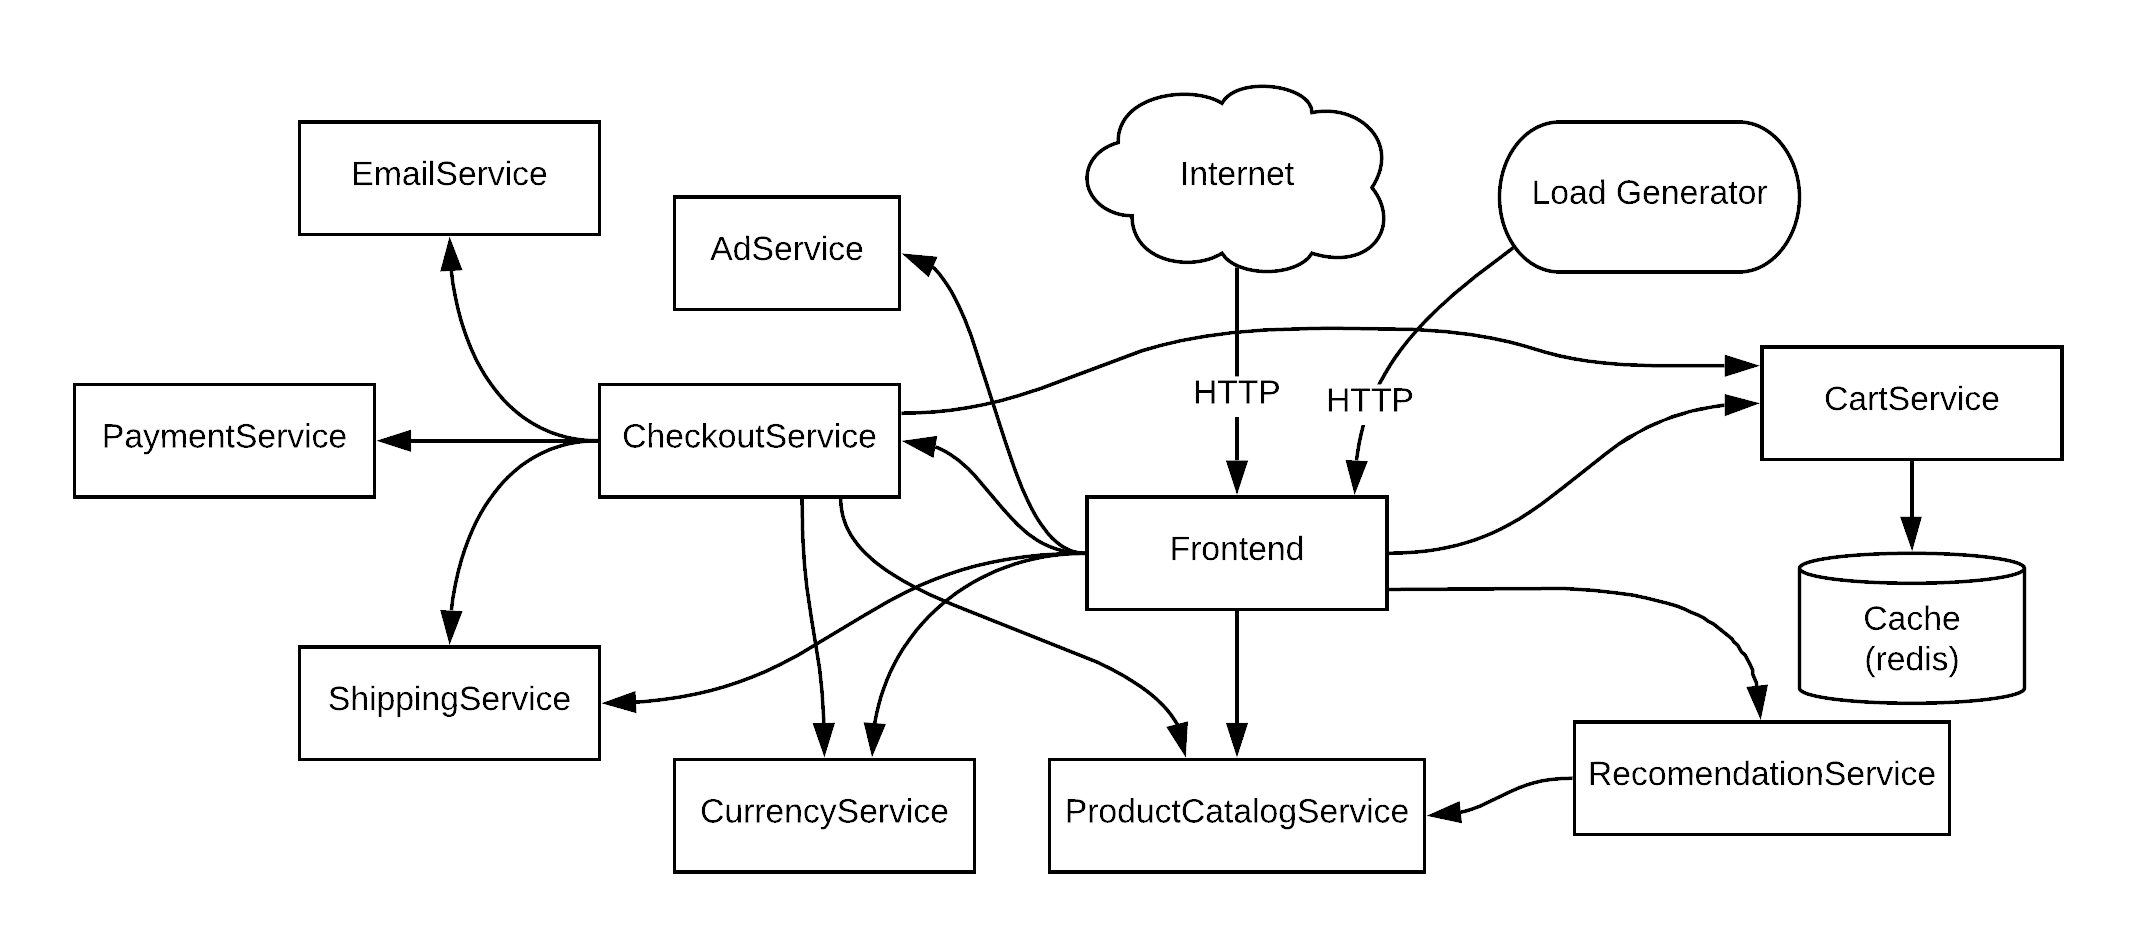
\includegraphics[width=15cm]{architecture-diagram.png}}
\caption{معماری برنامه فروشگاه آنلاین}
\label{fig:arch}
\end{figure}

\begin{table}
    \caption{توضیح میکرویس‌های فروشگاه آنلاین}
    \label{tab:microservices}
    \centering
    \begin{tabular}{|l|l|l|}
    \hline
        سرویس & زبان برنامه‌نویسی & توضیحات \\ \hline
        Frontend & Go & رابط کاربری \\ \hline
        CartService & C\# & ذخیره سبد خرید \\ \hline
        ProductCatalogService	 & Go & اطلاعات کالاها \\ \hline
        CurrencyService & Node.js & تبدیل ارز‌های مختلف \\ \hline
        PaymentService & Node.js & پرداخت \\ \hline
        ShippingService & Go & تعیین هزینه ارسال و ارسال کالا \\ \hline
        EmailService & Python & ارسال ایمیل \\ \hline
        CheckoutService & Go & ثبت سفارش \\ \hline
        RecommendationService & Python & پیشنهاد کالا \\ \hline
        AdService & Java & ارائه تبلیغات \\ \hline
        LoadGenerator & Python/Locust & ایجاد ترافیک \\ \hline
    \end{tabular}
\end{table}
ما درستی‌سنجی و تعریف قراردادها را روی میکروسرویس‌های 
\lr{CheckoutService}،
\lr{ShippingService}
و
\lr{ProductCatalogService}
که با زبان
Go
نوشته شده بودند انجام دادیم
\cite{forkedMicroservicesDemo}
و در نهایت توانستیم سه اشکال در این میکروسرویس‌ها پیدا کنیم.

\subsection{
سرویس CheckoutService
}

\singlespacing
\begin{figure}
	\begin{LTR}
		\lstinputlisting[language=protobuf2, breaklines=true, basicstyle=\ttfamily\footnotesize, caption={سرویس CheckoutService}, label={code:CheckoutProto}]{checkout.proto}
	\end{LTR}
\end{figure}
\doublespacing

این سرویس وظیفه ثبت سفارش را بر عهده دارد و توصیف رابط آن در برنامه
\ref{code:CheckoutProto}
آمده است. شرط‌های زیر را در یک قرارداد برای فرخوانی
\lr{\texttt{PlaceOrder}}
تعریف کردیم.

پیش‌شرط‌ها:
\begin{enumerate}
\item
ایمیل کاربر معتبر باشد.
\item
کارت اعتباری کاربر معتبر باشد.
\item
احراز هویت کاربر تایید شده باشد.
\end{enumerate}

پس‌شرط‌ها:
\begin{enumerate}
\item
در صورت موفقیت‌آمیز بودن خروجی تابع
\lr{\texttt{PlaceOrder}}
، باید تابع
\lr{\texttt{Charge}}
در
\lr{\texttt{PaymentService}}
با موفقیت فراخوانی شده باشد.
\item
تابع
\lr{\texttt{Charge}}
باید قبل از تابع
\lr{\texttt{ShipOrder}}
فراخوانی شده باشد.
\end{enumerate}

پیش‌شرط‌های ۱ و ۲ سبب پیدا شدن دو اشکال در برنامه شدند. چرا که بررسی درستی این مقادیر در رابط کاربری صورت می‌گرفت و در صورت فراخوانی مستقیم
\lr{API}ها
می‌شد داده نامعتبر به برنامه داد و برنامه نیز آن‌ها را قبول می‌کرد.


\subsection{
سرویس ShippingService
}

\singlespacing
\begin{figure}
	\begin{LTR}
		\lstinputlisting[language=protobuf2, breaklines=true, basicstyle=\ttfamily\footnotesize, caption={سرویس ShippingService}, label={code:ShippingProto}]{shipping.proto}
	\end{LTR}
\end{figure}
\doublespacing

این سرویس وظیفه ارسال سفارش را بر عهده دارد و توصیف رابط آن در برنامه
\ref{code:ShippingProto}
آمده است. شرط‌های زیر را در یک قرارداد برای فرخوانی
\lr{\texttt{ShipOrder}}
تعریف کردیم.

پیش‌شرط‌ها:
\begin{enumerate}
\item
تعداد کالاهای از یک نوع باید نامنفی باشد.
\end{enumerate}

پس‌شرط‌ها:
\begin{enumerate}
\item
در صورت موفقیت‌آمیز بودن خروجی تابع
\lr{\texttt{ShipOrder}}
مقدار
\lr{\texttt{TrackingId}}
در خروجی نباید خالی باشد.
\end{enumerate}

پیش‌شرط ۱ باعث پیدا شدن یک اشکال دیگر در برنامه شد، چرا که بررسی این شرط در برنامه به‌هیچ وجه انجام نمی‌شد.

\subsection{
سرویس ProductCatalogService
}

این سرویس وظیفه برگرداندن اطلاعات یک کالا را دارد و توصیف رابط آن در برنامه
\ref{code:ProductProto}
آمده است. شرط‌های زیر را در یک قرارداد برای فراخوانی
\lr{\texttt{GetProduct}}
تعریف کردیم.

پس‌شرط‌ها:
\begin{enumerate}
\item
مقدار ID در درخواست باید با مقدار ID در کالای برگردانده‌شده برابر باشد.
\end{enumerate}

\singlespacing
\begin{figure}
	\begin{LTR}
		\lstinputlisting[language=protobuf2, breaklines=true, basicstyle=\ttfamily\footnotesize, caption={سرویس ProductCatalogService}, label={code:ProductProto}]{productcatalog.proto}
	\end{LTR}
\end{figure}
\doublespacing


\section{سربار کارایی}
ما برای بررسی میزان سرباری که کتابخانه‌مان ایجاد می‌کند، ترافیک مشابهی در دو حالت روی برنامه ایجاد کردیم. اول در حالتی که بررسی قراردادها انجام شود، و دیگر بدون اینکه قراردادی تعریف شود. برای ایجاد ترافیک، رفتار تعداد کاربران همزمان را روی این برنامه شبیه‌سازی کردیم و سپس میانه زمان پاسخگویی به یکی از فراخوانی‌ها را اندازه‌گیری کردیم. خروجی این آزمایش در تصویر
\ref{fig:performance}
آمده است. همان‌طور که مشخص است، سربار زمانی ایجاد کاملا ناچیز است. همینطور در آزمایش‌های ما سربار حافظه نیز مقدار بسیار کوچکی بود.

\begin{figure}[t]
\centering
\begin{tikzpicture}
\begin{axis}[
    ybar,
    enlargelimits=0.15,
    legend style={at={(0.5,-0.25)},
      anchor=north,legend columns=-1},
    ylabel={Latency median (ms)},
    xlabel={Number of concurrent users},
    symbolic x coords={16, 64, 256},
    xtick=data,
    nodes near coords,
    nodes near coords align={vertical},
    ]
\addplot 
	coordinates {(16, 38) (64, 39) (256, 78)};
\addplot 
	coordinates {(16, 36) (64, 38) (256, 76)};
\legend{With contracts, No contract}
\end{axis}
\end{tikzpicture}
\caption{مقایسه زمان پاسخگویی}
\label{fig:performance}
\end{figure}
		% فصل چهارم: نتایج
% !TeX root=../main.tex
\chapter{بحث و نتیجه‌گیری}
%\thispagestyle{empty} 
\section{جمع‌بندی}
در این تحقیق در گام نخست با زمینه تحقیق، اهداف پیگیری‌شده و کارهایی که سابقا در این زمینه انجام شده‌است آشنا شدیم. سپس مفاهیم پایه‌ای مربوط به تحقیق عنوان و بررسی شد. در ادامه راه روشی ارائه شد و پیاده‌سازی‌ و کتابخانه توسعه داده‌شده، معرفی شدند. در نهایت روش درستی‌سنجی پیشنهاد شده روی یک پروژه واقعی پیاده شد و دیدیم که چگونه توانستیم چندین اشکال در این پروژه پیدا کنیم. همینطور سربار روش ارائه شده را نیز از نظر زمانی و حافظه بررسی کردیم و دیدیم که این سربار بسیار ناچیز است.

\section{نتیجه‌گیری}
با توجه به نتایج به دست آمده، دیدیم که روش طراحی بر اساس قرارداد و درستی‌سنجی پویا روش مناسبی برای درستی‌سنجی نرم‌افزارهای با معماری میکروسرویس است. چرا که با استفاده از این روش، ارتباط بین میکروسرویس‌ و انتظارات هر سرویس به صورت دقیق بررسی می‌شود و در صورت نقض شدن هر کدام از انتظارات، توسعه‌دهنده به سرعت متوجه خواهد شد.

\section{دست‌آورد‌ها}
ما در این تحقیق توانستیم از میان روش‌های موجود، روشی مناسب را برای درستی‌سنجی میکروسرویس‌ها انتخاب کنیم و آن را با توجه به این نیازمندی، بهینه کنیم. سپس یک پیاده‌سازی برای این روش ارائه دادیم و با درستی‌سنجی یک پروژه واقعی، کارایی آن را در عمل بررسی کردیم. یکی از دست‌آوردهای اصلی این تحقیق، امکان نوشتن شرط روی ترتیب اجرای فراخوانی‌های از راه دور است که به درستی‌سنجی ارتباط بین میکروسرویس‌ها کمک شایانی خواهد کرد.

\section{محدودیت‌ها}
در حال حاضر، محدودیت اصلی کتابخانه نوشته شده، وابسته بودن آن به تکنولوژی‌های انتخاب شده است و اگر سرویسی از تکنولوژی‌های دیگری استفاده کند، نمی‌توان از این کتابخانه استفاده کرد. همینطور در مقیاس‌های بسیار بزرگ ممکن است سربار زمانی زیاد شود که با توجه به محدودیت امکانات، این مورد را نتوانستیم بررسی کنیم.

\section{پیشنهادها}
برای ادامه این تحقیق، خوب است امکان این در نظر گرفته شود که سرویس‌هایی که با تکنولوژی‌های مختلف نوشته می‌شوند، بتوانند از کتابخانه ارائه شده استفاده کنند. همین‌طور واسط کتابخانه معرفی شده بسیار جای بهبود دارد و می‌توان قابلیت‌های خیلی بیشتری به آن اضافه کرد. همچنین می‌توان روی تحلیل رسمی روش ارائه شده کار کرد و آن را دقیق ارائه داد.
		% فصل پنجم: بحث و نتیجه‌گیری

% مراجع
% اگر از استیل‌های natbib استفاده می‌کنید باید دو خط را در فایل commands.tex تغییر دهید.
\pagestyle{empty}
{
\small
\onehalfspacing
\bibliographystyle{plain-fa} % or plainnat-fa for author-date
\bibliography{./tex/MyReferences}
}

\pagestyle{fancy}

% \appendix
% فصلهای پس از این قسمت به عنوان ضمیمه خواهند آمد.

% دستورات لازم برای تبدیل «فصل آ» به «پیوست آ» در فهرست مطالب
\addtocontents{toc}{
    \protect\renewcommand\protect\cftchappresnum{\appendixname~}%
    \protect\setlength{\cftchapnumwidth}{\mylenapp}}
    
\let\Chapter\chapter
% دستورات لازم برای شماره‌گذاری صفحات پیوست‌ها بشکل آ-۱ (فعلا با glossaries سازگار نیست)
%\pretocmd{\chapter}{
%  \clearpage
%  \pagenumbering{arabic}
%  \renewcommand*{\thepage}{\rl{\thechapter-\arabic{page}}}}{}{}
%%%%%%%%%%%%%%%%%%%%%%%%%%%%%%%%%%%%%
    

\include{./tex/appendix1}		% پیوست اول: آشنایی مقدماتی با لاتک
\include{./tex/appendix2}		% پیوست دوم: جدول، نمودار و الگوریتم در لاتک
\include{./tex/appendix3}   	% پیوست سوم: مراجع، واژه‌نامه و حاشیه‌نویسی

% برگرداندن شماره‌بندی صفحات فصول
\let\chapter\Chapter
\pagenumbering{tartibi} % اول، دوم، ...
%\baselineskip=.75cm

% چاپ واژه‌نامه‌ها و نمایه 
\onehalfspacing
\printglossary
\printindex

\begin{latin}
\baselineskip=.6cm
\latinTitlePage
\end{latin}
\label{LastPage}

\end{document}
